\documentclass[11pt]{article}
\renewcommand{\baselinestretch}{1.8}
\usepackage{textcomp}
\usepackage{fontenc}
\usepackage{graphicx}
\usepackage{caption} % for Fig. captions
\usepackage{gensymb} % for \degree
\usepackage{placeins} % for \images
\usepackage[margin=1in]{geometry} % to set margins
\usepackage{setspace}
\usepackage{lineno}
%\usepackage{cite}
\usepackage{amssymb} % for math symbols
\usepackage{amsmath} % for aligning equations
\usepackage{natbib}
\renewcommand{\thetable}{S\arabic{table}}
\renewcommand{\thefigure}{S\arabic{figure}}
\usepackage{xr-hyper}
\externaldocument{new_sensitivity}

\bibliographystyle{..//..//sub_projs/refs/styles/besjournals.bst}

\linenumbers
\title{Supporting Information: Differences in flower and leaf bud responses to the environment drive shifts in spring phenological sequences of temperate woody plants}

\date{}
\author{D.M. Buonaiuto $^{1,2,a}$, E.M. Wolkovich$^{3}$}

\begin{document}
\maketitle

\section*{Tables}


\begin{table}[!ht]
\begin{tabular}{cccc}
  \hline
 Chilling\_model & Harvard Forest Mean (sd) & Chamber: 30 days & Chamber: 60 days \\ 
  \hline
 Utah Model & 979.64  (248.34) & 720.00 & 1440.00 \\ 
Chill Hours & 1170.71 (273.07) & 720.00 & 1440.00 \\ 
 Dynamic Model & 86.56 ( 16.64) & 21.25 & 43.50 \\ 
   \hline
\end{tabular}
\caption{\textbf{Comparisons between chilling treatments applied in our experiment to the average chilling at our sampling site (Harvard Forest in Petersham, MA)  are sensitive to the way chilling is calculated.} We used daily temperature data from Harvard Forest \citep{} to calculate average field chilling from October 15-April 15 over a 20 year period using three different chilling models. The Utah and Chilling hours models suggest the average chilling at our sampling site is between our two experimental chilling treatments, while the dynamic models suggests that field chilling is generally higher than either of our experiment treatments. Should add a sentence about why.}
\label{tab:chillcomps}
\end{table}

\begin{table}[!ht]
\centering
\begin{tabular}{|r|r|r|r|r|r|}
  \hline
 & Estimate & Est.Error & Q25 & Q75 & phase \\ 
  \hline
Intercept & 77.54 & 10.01 & 70.91 & 84.01 & flower \\ 
 & 70.30 & 8.93 & 64.56 & 76.01 & budburst \\ 
  \hline
  Chill & -21.31 & 7.54 & -26.14 & -16.78 & flower\\ 
   & -30.35 & 5.20 & -33.66 & -27.06 & budburst\\ 
 \hline
  Light & -5.99 & 5.83 & -9.73 & -2.12 & flower\\ 
   & 5.95 & 5.12 & 2.68 & 9.29 & budburst\\ 
  \hline
  Force & -18.87 & 6.36 & -22.85 & -14.85 & flower\\ 
 & -17.39 & 5.16 & -20.70 & -14.01 & budburst \\ 
  \hline
  Chill:Light & -0.70 & 6.17 & -4.60 & 3.44 & flower\\ 
     & -5.04 & 4.16 & -7.73 & -2.26 & budburst\\ 
  \hline
  Chill:Force & 6.75 & 6.62 & 2.73 & 10.96 & flower \\ 
   & 12.31 & 4.77 & 9.28 & 15.42 & budburst \\ 
  \hline
  Light:Force & -5.42 & 6.22 & -9.39 & -1.30 & flower \\ 
    & -12.90 & 4.12 & -15.54 & -10.17 & budburst\\ 
   \hline
\end{tabular}
\caption{\textbf{Model estimates of the effect of variation in chilling, forcing and photoperiod on the flower and leaf phenology of 10 temperate woody plant species suggest that the strength of phenological responses to environmental change is phase specific.}}
\label{tab:modelests}
\end{table}

\pagebreak


\pagebreak
\pagebreak

%\section*{Figures}
   %\begin{figure}[h!]
    %\centering
 %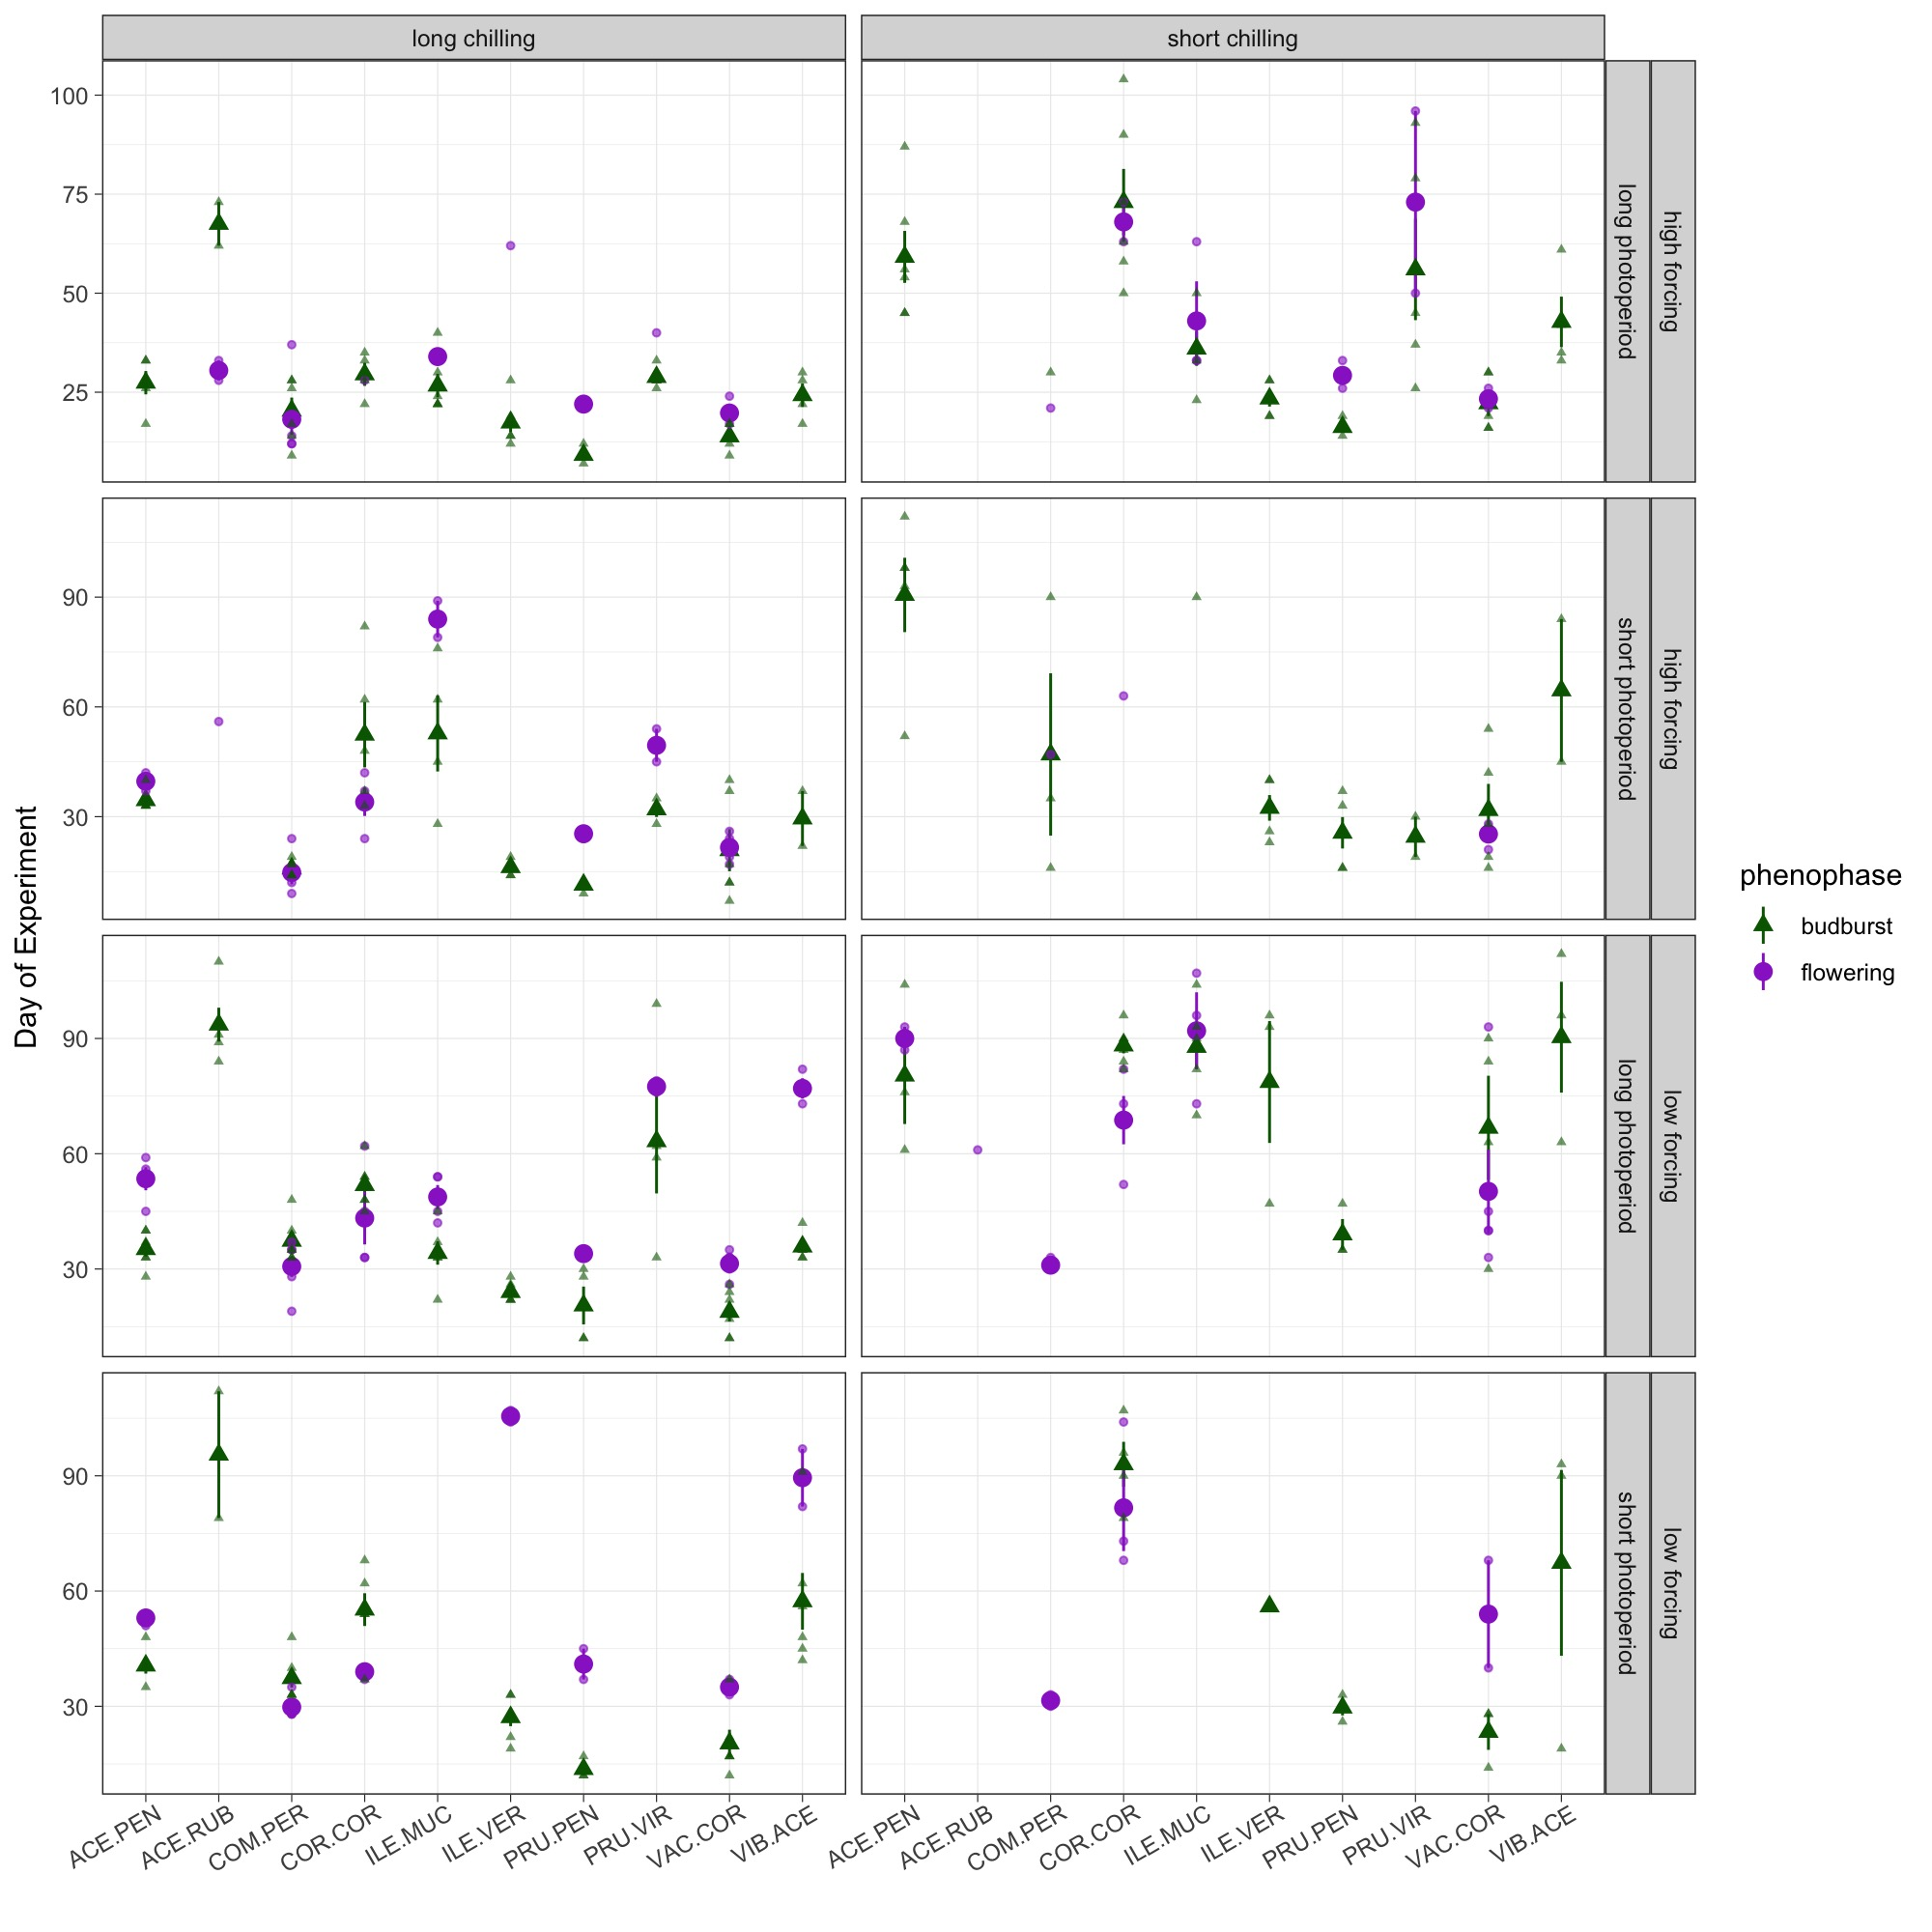
\includegraphics[width=\textwidth]{..//Plots/rawdataplots.jpg}
  %  \caption{\textbf{Observed day of leaf budburst and flowers open for 10 temperate woody species under eight environmental treatment combinations.} The larger shapes and lines show the mean and standard error for each phenophase/species/treatment with the smaller lighter shape showing individual level data for every individual in the experiment. FLS variation among treatments was high and varied considerably by species.}
   % \label{fig:raw}
%\end{figure}

  \begin{figure}[!ht]
    \centering
 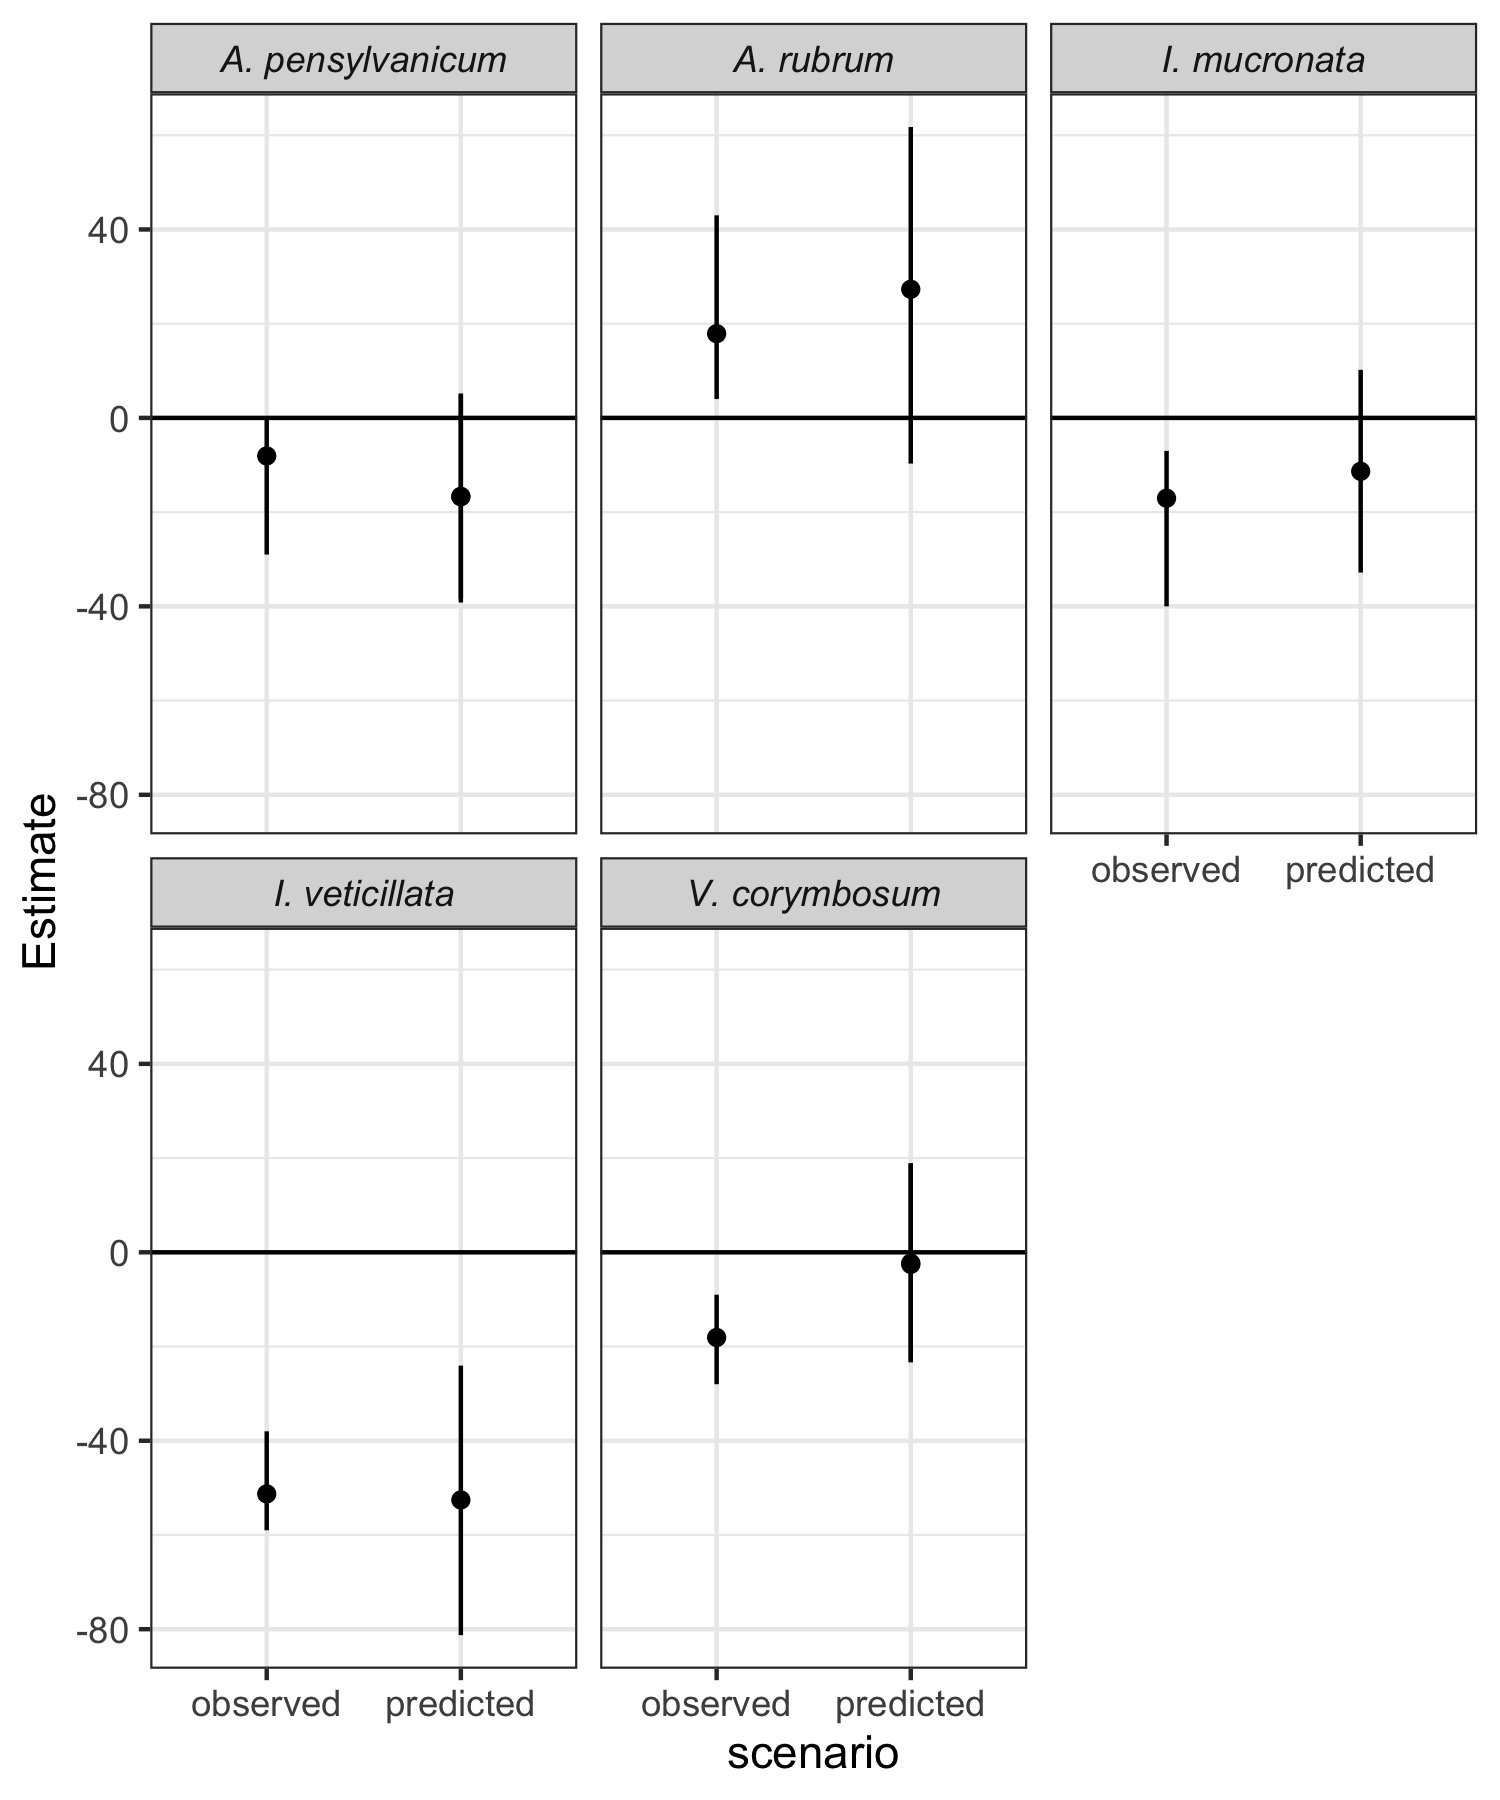
\includegraphics[width=\textwidth]{..//Plots/fieldmodcomparisions.jpeg}
    \caption{\textbf{Model predictions of flower-leaf sequence interphases (days between phenophase) under artificial conditions designed to approximate ``average" field conditions reflect FLS interphases observed at Harvard Forest in Pertersham MA.}. This comparison suggest that the baseline environmental treatments  applied in our experiment appropriately capture natural conditions. Dot represent means FLS interphase in both datasets, and lines represent the 89\% credible intervals and the full range of observations for our model predictions and Harvard Forest data respectively.  Harvard Forest phenological records are from \citet{Okeefe2015}.}
    \label{fig:validate}
\end{figure}
\pagebreak

\section*{Simulations}
\noident To better understand the patterns of phenological sensitivity generated by the precocity hierarchy hypothesis (PHH) and the differential sensitivity hypothesis (DSH) respectively, we mathematically simulated the underlying physiology of each hypothesis, and these simulations to generate flower and leaf phenology under two levels of chilling, forcing and photoperiod in a fully factorial simulation.\\

\noindent For the PHH we assigned flowering and leafing a critical heat sum threshold (F*) above which the phenological event would take place. We did this using a growing degree model with a base temperature of 5\degree C \citep{}. For the PHH simulations, we assigned flowering an F* of 200 GDDs and leafing an F* of 400 GDDs. In this scenario we let increased both chilling and photoperiod reduce the F* value for each phenophase by 100 and 20 respectively.\\

\noindent For the DSH we assigned flowering and leafing identical F* values of 400. As in the previous scenario, we let increased chilling and photoperiod reduce the F* values, but these cues reduced the F* for leafing by 200 and 0 respectively and for flowering by 100 and 20.

\noindent We also included a third scenario that included both initial F* differences of the PHH (flowering: 200 and leafing: 400) and the differential response to chilling and photoperiod of the DSH (flowering: -100 chilling, -20 photoperiod, leafing -200 chilling, 0 photoperiod).

\bibliography{..//..//sub_projs/refs/hyst_outline.bib} 
\end{document}
